\documentclass[aspectratio=169]{beamer}
\usepackage{beamerthemeCOOP}
%packages%
%\usepackage{savesym}
%\usepackage{longtable}
%\usepackage{listings}
%\usepackage{placeins}
%\usepackage[font=itshape,noorphans=true]{quoting}

%font
\usepackage{amsmath,amsfonts,amsthm,amssymb,mathtools,stmaryrd,xpatch}
%\usepackage[T1]{fontenc}
%\usepackage{libertine}
%\usepackage{kpfonts}
%\usepackage[libertine]{newtxmath}

\usepackage{appendixnumberbeamer}
\usepackage{quoting}
\usepackage{csquotes}
\usepackage{color}
\usepackage{listings}
\usepackage[hang]{subfigure}
\usepackage[english]{babel}
\usepackage{tikz}
\usepackage[vlined,linesnumbered,resetcount]{algorithm2e}
\usepackage{enumitem}
\usepackage{framed}
\usepackage[capitalise]{cleveref}
\usepackage{apacite}
%\usepackage[numbers,sort]{natbib}
\usepackage{svg}
%\usepackage[utf8]{inputenc}
\usepackage{hyperref}
\hypersetup{colorlinks,linkcolor=mucdaiblue,citecolor=,urlcolor=mucdaiblue}
\usepackage{etoolbox}% http://ctan.org/pkg/etoolbox
\usepackage{array}
\usepackage{pbox}
\usepackage[export]{adjustbox}

\input{meta}
\input{commands}
\usepackage{graphicx}

\definecolor{midnightblue}{RGB}{10,10,44}
\definecolor{navyblue}{RGB}{0,0,120}
\definecolor{crimson}{RGB}{220,20,60}
\definecolor{mydarkgray}{RGB}{33,33,33}
\definecolor{myalgColor}{RGB}{99,99,99}
\definecolor{mygreen}{RGB}{85,168,104}
\definecolor{myorange}{RGB}{221,132,82}
\definecolor{myblue2}{rgb}{0.12156862745098039, 0.4666666666666667, 0.7058823529411765}
\definecolor{myblue3}{rgb}{0.2980392156862745, 0.4470588235294118, 0.6901960784313725}
\definecolor{myblue4}{rgb}{0.2823529411764706, 0.47058823529411764, 0.8156862745098039}
\definecolor{mybluebright}{rgb}{0.00784313725490196, 0.24313725490196078, 1.0}
\definecolor{myred}{RGB}{196,78,82}
\definecolor{mydarkgray}{RGB}{90,90,90}
\definecolor{mygray}{RGB}{179,179,179}
\definecolor{myviolet}{RGB}{129,114,178}
\definecolor{myblue}{RGB}{76,114,202}
\xdefinecolor{mybg}{rgb}{0.7419607843137255, 0.9027297193387159, 0.868958093041138}
\xdefinecolor{myRed}{rgb}{0.7686274509803922, 0.3058823529411765, 0.3215686274509804}
\xdefinecolor{prevColor}{rgb}{0.39215686274509803, 0.7098039215686275, 0.803921568627451}
\xdefinecolor{hmred}{RGB}{228, 24, 58}
\xdefinecolor{mylightblue}{rgb}{0.8584083044982699, 0.9134486735870818, 0.9645674740484429}

\definecolor{mybrightblue}{rgb}{0.00784313725490196, 0.24313725490196078, 1.0}
\definecolor{mybrightred}{rgb}{0.9098039215686274, 0.0, 0.043137254901960784}

\xdefinecolor{myalgColor}{rgb}{0.7686274509803922, 0.3058823529411765, 0.3215686274509804}

\definecolor{mucdaibackground}{HTML}{03001B}
\definecolor{mucdaiblue}{HTML}{3E46D9}
\definecolor{mucdaipurple}{HTML}{6100ff}
\definecolor{mucdaipurpledark}{RGB}{47,16,157}

\definecolor{p5keywordstyle}{HTML}{d52889}
\definecolor{p5identifierstyle}{HTML}{7a5a3a}
\definecolor{p5ndkeywordstyle}{HTML}{0b7ca9}
%\definecolor{p5ndkeywordstyle}{HTML}{7a5a3a}
\definecolor{p5stringstyle}{HTML}{47820a}
\definecolor{p5background}{HTML}{FFFFFF}
\definecolor{p5basicstyle}{HTML}{333333}

\definecolor{p5darkkeywordstyle}{HTML}{ffa9d9}
\definecolor{p5darkidentifierstyle}{HTML}{f5dc23}
\definecolor{p5darkndkeywordstyle}{HTML}{00FFFF}
%\definecolor{p5ndkeywordstyle}{HTML}{7a5a3a}
\definecolor{p5darkstringstyle}{HTML}{2de9b6}
\definecolor{p5darkbackground}{HTML}{333333}
\definecolor{p5darkbasicstyle}{HTML}{fdfdfd}


%%% Title page %%%
%\defbeamertemplate*{title page}{customized}[1][]
%{
%	\usebeamerfont{title}\inserttitle\par
%	\usebeamerfont{subtitle}\usebeamercolor[fg]{subtitle}\insertsubtitle\par
%	\bigskip
%	\usebeamerfont{author}\insertauthor\par
%	\usebeamerfont{institute}\insertinstitute\par
%	\usebeamerfont{date}\insertdate\par
%	\usebeamercolor[fg]{titlegraphic}\inserttitlegraphic
%}
\title{\Huge Creative Coding mit p5.js}
%\subtitle{Creative Coding mit p5.js}
\author{Dr. Benedikt Zönnchen \\\scriptsize zoennchen.benedikt@hm.edu} 
\date{23. September 2024}
\institute{%
	%Hochschule München\\ \vspace{5mm}%
	\includegraphics[height=20pt]{./figs/logo/Hochschule_Muenchen_Logo}
	\hspace{2mm}
	
\includegraphics[height=20pt]{./figs/logo/MUC_DAI_Logo_RGB_Weiss.pdf}}
%%% End Title page %%%
\setbeamercovered{transparent}

\begin{document}
\begin{frame}[plain]
	\titlepage
\end{frame}

\begin{frame}
	\frametitle{Was ist Creative Coding?}
	\begin{block}{Definitionsversuch}
	\enquote{Creative Coding ist ein \alert{Prozess} der auf \alert{Erkundung}, \alert{Wiederholung}, \alert{Reflexion} und \alert{Entdeckung} basiert und bei dem Code als primäres Medium genutzt wird, um eine diverse Menge an Artefakten zu erzeugen.} -- \cite{mitchell:2013}
	\end{block}
\end{frame}

\begin{frame}
	\frametitle{Persönliche Artefakte}
	\begin{columns}
		\begin{column}{0.3\textwidth}
		\fbox{\includegraphics[height=0.5\textheight]{./figs/noisy_circles}}
		\end{column}
		\hfill
		\begin{column}{0.3\textwidth}
		\fbox{\includegraphics[height=0.5\textheight]{./figs/red-flake-4}}
		\end{column}
		\hfill
		\begin{column}{0.4\textwidth}
		\fbox{\includegraphics[height=0.5\textheight]{./figs/fractal_tree}}
		\end{column}
	\end{columns}
\end{frame}

\begin{frame}
	\frametitle{Professionelle Artefakte}
	\begin{center}
	\begin{columns}
		\begin{column}{0.3\textwidth}
		\fbox{\includegraphics[height=0.5\textheight]{./figs/manolo_gamboa_naon}}
		Manolo Gamboa Naon
		\end{column}
		\hfill
		\begin{column}{0.3\textwidth}
		\fbox{\includegraphics[height=0.5\textheight]{./figs/mark_j_stock}}
		Mark J. Stock
		\end{column}
		\hfill
		\begin{column}{0.3\textwidth}
		\fbox{\includegraphics[height=0.5\textheight]{./figs/anders_hoff}}
		Anders Hoff
		\end{column}
	\end{columns}
	\end{center}
\end{frame}

\begin{frame}
	\frametitle{Was ist p5.js?}
	\begin{enumerate}[label=$\bullet$]
		\item \textit{\href{https://p5js.org/}{p5.js}} ist eine Open Source JavaScript Bibliothek für \alert{Creative Coding}
		\item Basiert auf \textit{\href{https://processing.org/}{Processing}}
		\item Initiatorin: Lauren McCarthy, siehe \cite{mccarthy:2015}
		\item \alert{Ziel}: Das Programmieren von (professionellen) interaktiven, grafischen Anwendungen so einfach wie möglich zu machen.
	\end{enumerate}
    
\end{frame}



\begin{frame}
	\frametitle{Was ist Creative Coding?}
    \begin{center}
    \Huge Demo!
    \end{center}
\end{frame}

\begin{frame}
	\frametitle{Was ist Creative Coding?}
    %\def\svgwidth{\columnwidth}
    %\scalebox{0.5}{\input{./figs/cycle.pdf_tex}}
    \begin{figure}
    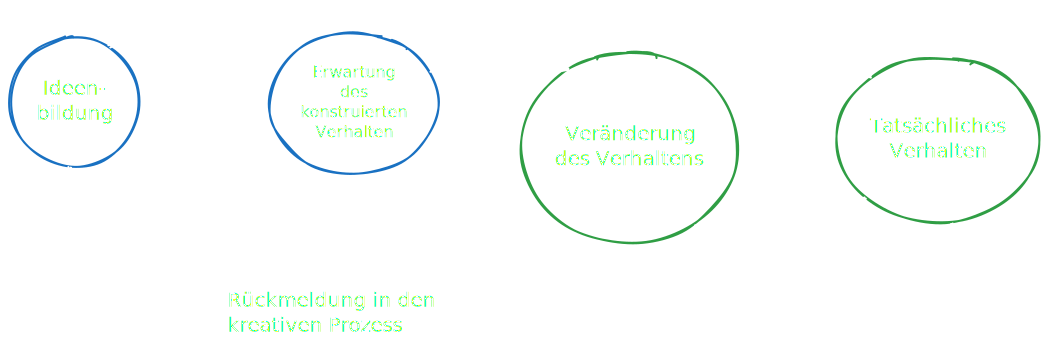
\includegraphics[width=\textwidth]{./figs/cycle.png}
    \caption{Tweak/Run/Observe Feedback Loop, Quelle: \cite{mitchell:2013}}
    \end{figure}
\end{frame}

\begin{frame}[fragile]
\frametitle{Creative Coding als Prozess}
Zeichne eine Linie von links unten quer über die Leinwand.
{\color{p5darkbasicstyle}
\begin{lstlisting}
line(width,0,0,height);
\end{lstlisting}
  }

  \begin{center}
  	\fbox{\includegraphics[height=0.45\textheight]{./figs/line}}
  \end{center}
\end{frame}

\begin{frame}[fragile]
\frametitle{Creative Coding als Prozess}
Zeichne eine Linie zufällig quer über die Leinwand.

{\color{p5darkbasicstyle}
\begin{lstlisting}
if(random() > 0.5) {
	line(0,0,width,height);
}
else {
	line(width,0,0,height);
}
\end{lstlisting}
}

  \begin{center}
  	\fbox{\includegraphics[height=0.45\textheight]{./figs/line}}
  	\hspace{1cm}
  	\fbox{\includegraphics[height=0.45\textheight]{./figs/line2}}
  \end{center}
\end{frame}


\begin{frame}[fragile]
\frametitle{Creative Coding als Prozess}
Zeichne eine Linie zufällig quer über die Leinwand.\\
Wiederhole den Prozess für viele nebeneinander liegende Leinwände!
\begin{columns}
\begin{column}{0.5\textwidth}
{\color{p5darkbasicstyle}
\begin{lstlisting}
let dx = width / n;
let dy = height / n;
  
for(let i = 0; i < n; i++){
 for(let j = 0; j < n; j++) {
  if(random() > 0.5) {
   line(dx * i, dy * j, 
    dx * (i+1), dy * (j+1));
  }
  else {
   line(dx * (i+1), dy * j, 
    dx * i, dy * (j+1));
  }
 }
} 
\end{lstlisting}
}
\end{column}
\begin{column}{0.5\textwidth}
\fbox{\includegraphics[height=0.66\textheight]{./figs/tilling}}
\end{column}
\end{columns}
\end{frame}

\begin{frame}
	\frametitle{Wie funktioniert p5.js?}
    %\def\svgwidth{\columnwidth}
    %\scalebox{0.5}{\input{./figs/cycle.pdf_tex}}
    \begin{figure}
    \includegraphics[width=\textwidth]{./figs/p5-draw-cycle.png}
    \end{figure}
\end{frame}

\begin{frame}
	\frametitle{Was ist Creative Coding?}
	\begin{block}{Definitionsversuch}
	\enquote{Creative Coding ist ein \alert{Prozess} zur \alert{Reflexion} über und \alert{Erkundung} bzw. \alert{Entdeckung} von \alert{Algorithmen}/Code.}
	\end{block}
\end{frame}

\begin{frame}
	\frametitle{Was ist Creative Coding?}
\begin{center}
	\enquote{Im \alert{Creative Coding} geht es um \alert{freie Exploration}. [...] es ist eine \alert{Reflexion über die Technik} selbst. [...] Anders als in der klassischen Programmierung sind beim Creative Coding Fehler nicht ärgerlich, sondern gern gesehen, denn häufig erzeugen sie spannende Ergebnisse, leiten eine Idee in neue Richtungen und mich Schritt für Schritt an ein Ziel, das ich niemals festgelegt habe. Dieser Prozess an sich ist sehr kreativ.}\\-- \cite{huebner:2023}
	\end{center}
\end{frame}

\begin{frame}
	\frametitle{Was ist Creative Coding?}
    %\def\svgwidth{\columnwidth}
    %\scalebox{0.5}{\input{./figs/cycle.pdf_tex}}
    \begin{figure}
    \includegraphics[width=\textwidth]{./figs/cycle2.png}
    \end{figure}
\end{frame}

%\begin{frame}
%	\begin{quoting}
%		\enquote{\textit{Unsere Zukunft ist eine spannende, die das Analoge und Digitala, Mensch und Maschine vereint, anstatt das eine auf Kosten des anderen zu bevorzugen.}}\\-- Jason Baley
%	\end{quoting}
%	\vspace{0.5cm}
%	\begin{quoting}
%		\enquote{\textit{Das Digitale ist nicht hier, um etwas zu beenden. Vielmehr ist es da, um alles zu erweitern, zu kombinieren und mehr Dinge erreichbar zu machen. Für Künstler:innen ist es die innovativste Arbeit von allen; die größte und aufregendste Herausforderung in einer langen Geschichte der Synthese zwischen Technologie, Hand, Geist und Herz.}}\\-- J.D. Jarvis
%	\end{quoting}
%\end{frame}

\begin{frame}
	\frametitle{Was ist Creative Coding?}
	\begin{center}
	\enquote{Generative art is truly working with the essence of what shapes our new digital worlds. Coding is the key. Our future lives will be built with it. The artistic exploration of code and how it can be re-imagined, re-examined, and re-purposed is critical if we wish to build a healthy, human experience in the non-physical landscapes to come.}\\-- \cite{hobbs:2021}
	\end{center}
\end{frame}


\begin{frame}
	\frametitle{Ressourcen \& Inspirationsquellen}
	\begin{enumerate}[label=$\bullet$]
		\item Sammlung allgemeiner Ressourcen: \textit{\href{https://github.com/terkelg/awesome-creative-coding}{Awesome Creative Coding}}
		\item Plattform zum Teilen von p5.js Sketches: \textit{\href{https://openprocessing.org}{OpenProcessing}}
		\item Künstler: \textit{\href{https://www.brunoimbrizi.com}{https://www.brunoimbrizi.com}}
		\item ...
	\end{enumerate}
\end{frame}

\appendix

%ODO: plot different d_Gamma
\begin{frame}[plain,allowframebreaks]
	\frametitle{Literatur}
	{\scriptsize% dirty fix for the non-chapter bib
		\bibliographystyle{apacite}
		\bibliography{Literature}}
\end{frame}

\end{document}
